\documentclass[10pt,a4paper]{article}
\usepackage[a4paper,margin=2cm]{geometry}
\usepackage[T1]{fontenc}
\usepackage{newtxtext,newtxmath}
\usepackage{microtype}
\usepackage{graphicx}
\usepackage{booktabs}
\usepackage{multirow}
\usepackage{xcolor}
\usepackage[font=small,labelfont=bf,skip=3pt]{caption}
\usepackage{enumitem}
\usepackage{titlesec}
\usepackage[section]{placeins}  % keep floats inside their section
\usepackage[numbers,sort&compress]{natbib}
\usepackage[colorlinks=true,linkcolor=black,citecolor=black,urlcolor={blue!60!black}]{hyperref}

\titlespacing*{\section}{0pt}{7pt plus 2pt}{3pt}
\titlespacing*{\subsection}{0pt}{5pt plus 2pt}{2pt}
\titleformat*{\section}{\large\bfseries}
\titleformat*{\subsection}{\normalsize\bfseries}
\setlength{\parskip}{2pt}
\setlist{nosep,leftmargin=1.2em}
\setlength{\textfloatsep}{8pt plus 2pt}
\setlength{\floatsep}{6pt plus 2pt}
\setlength{\abovecaptionskip}{3pt}
\renewcommand{\topfraction}{0.9}
\renewcommand{\bottomfraction}{0.8}
\renewcommand{\textfraction}{0.07}
\renewcommand{\floatpagefraction}{0.85}
\setcounter{topnumber}{3}
\setcounter{totalnumber}{4}
\newcommand{\obs}{\textsc{obs}}
\newcommand{\hyp}{\textsc{hyp}}

\title{\vspace{-1.2cm}\Large\textbf{DSA4213 Assignment 1: Language Models, Embeddings and Representations}}
% Personal details live in private/author.tex, which is not in the repository; the public build is anonymous.
% Personal build: latexmk -pdf -outdir=private -jobname=<name> -usepretex='\def\withauthor{1}' report.tex
\ifdefined\withauthor
  \input{private/author}
\else
  \newcommand{\reportauthor}{Anonymous submission}
\fi
\author{\reportauthor\\ \small Code: \url{https://github.com/XenonLyn/assignment-dsa4213}}
\date{\vspace{-0.6cm}}

\begin{document}
\maketitle

\noindent\textbf{Comparison question.} \emph{On one small corpus and a fixed training budget, how do
n-gram, RNN, LSTM and Transformer language models differ; do fixed pre-trained input embeddings help;
and does better next-token prediction give better representations for classification?}
Throughout, we label statements as observations (\obs) or hypotheses (\hyp); every number is from a
single run (seed 42) unless stated otherwise.

\section{Data and common setup}
\textbf{Corpus.} WikiText-2 \citep{merity2016}, tokenised version (\texttt{wikitext-2-v1}); 2.08M / 216k / 244k
train / validation / test tokens. Preprocessing: lower-casing (for GloVe coverage in Part~II), whitespace
tokens, an \texttt{<eos>} token at the end of every non-empty line. The vocabulary (28,913 types) is built
on the training split only; the dataset's own \texttt{<unk>} covers 2.6\% / 5.4\% / 6.2\% of train /
validation / test tokens and is scored like any other word (no further OOV words occur).
\textbf{Common evaluation.} Every split is cut into non-overlapping chunks of 128 targets; each target is
predicted from the preceding tokens \emph{inside its chunk only}, for every model including the n-gram
(no state is carried across chunks). Padded targets are excluded from the loss. Metric: mean next-token
cross-entropy (CE, nats) and perplexity PPL$=\exp(\text{CE})$. All selection (n-gram order, best epoch,
learning rate, classifier regularisation) uses validation data only; test data is used once per model.
\textbf{Hardware and budget.} Apple M1 laptop (8-core CPU, 16\,GB, fanless), PyTorch 2.5.1, neural models on
the MPS GPU backend, n-gram on CPU. Every neural model gets the same budget: 10 epochs = 5,070 updates of
32$\times$128 tokens, AdamW (weight decay 0.01), 200 warm-up steps then cosine decay to 10\% of the peak
learning rate (LR), gradient clipping at 1.0. Models are trained one at a time.

\section{Part I: four language models}
\textbf{Models} (details in Appendix~\ref{app:config}). \emph{n-gram}: interpolated Kneser--Ney
\citep{kneser1995,chen1999} with absolute discounts per order; orders 1--4 scored on validation (PPL 818 / 275 /
236 / 230), order 4 selected. \emph{RNN}: 2-layer tanh RNN, hidden 512. \emph{LSTM} \citep{hochreiter1997}: 2
layers, hidden 512. \emph{Transformer} \citep{vaswani2017}: decoder-only, 4 pre-LN blocks, $d{=}300$, 6 heads,
FFN 1200, learned positions, causal mask. All neural models use randomly initialised, trainable 300-d input
embeddings (chosen to match GloVe-300d for Part~II), an untied softmax layer, and dropout (0.3 RNN/LSTM, 0.2
Transformer) on the embeddings, between layers and before the softmax. A start-up test asserts that changing
future tokens never changes earlier outputs. Peak LR was chosen on validation from \{1e-3, 3e-3\} for the
recurrent models (RNN 1e-3: val PPL 228 vs 240; LSTM 3e-3: 148 vs 201); the Transformer used 5e-4 (one value).

\textbf{Cost measurement.} Training time sums the training loops only (validation excluded, device
synchronised). Inference uses one common workload for all models, re-timed back to back in one process:
scoring the whole test set under the common setup (batch 32) and generating 50 tokens for each of 5 prompts
(batch 1), one warm-up run, median of 3. The Transformer re-encodes its window at every generation step (no
KV cache); RNN/LSTM update their state.

\begin{table}[t]
\centering\small
\caption{Part I: prediction quality and cost (test set, common chunked setup). Params: total (non-embedding,
non-softmax body). Throughput in tokens/s; n-gram on CPU, neural models on the M1 GPU. Timing differences
below $\sim$10\% (training) or $\sim$25\% (inference) are within the noise we measured on this laptop.}
\label{tab:part1}
\begin{tabular}{lrrrrrr}
\toprule
Model & Size & Test CE & \textbf{Test PPL} & Train time & Scoring tok/s & Generation tok/s\\
\midrule
4-gram Kneser--Ney & 5.8M n-grams (81\,MB) & 5.379 & 216.7 & 5\,s & 301{,}407 & 470\\
RNN & 24.4M (0.94M) & 5.367 & 214.2 & 56\,min & 19{,}953 & 146\\
LSTM & 27.3M (3.77M) & \textbf{4.930} & \textbf{138.4} & 59\,min & 25{,}472 & 136\\
Transformer & 19.6M (2.21M) & 4.945 & 140.5 & 53\,min & 29{,}345 & 62\\
\bottomrule
\end{tabular}
\end{table}

\begin{figure}[t]
\centering
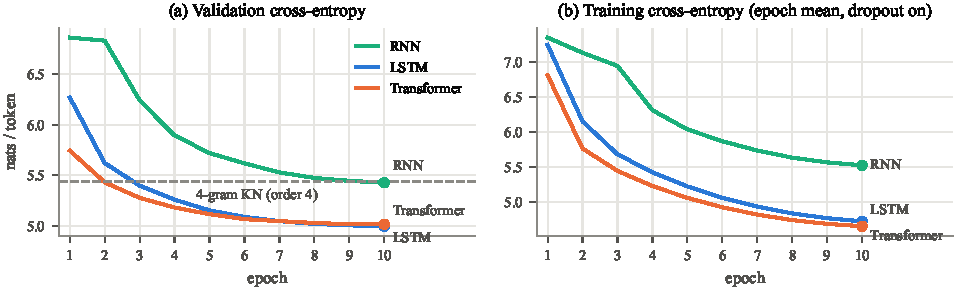
\includegraphics[width=\linewidth]{figures/fig1_part1_curves.pdf}
\caption{Part I learning curves. (a) Validation CE per epoch; dashed: 4-gram validation CE. (b) Training CE
(epoch average, with dropout active).}
\label{fig:part1}
\end{figure}

\textbf{Prediction quality} (Table~\ref{tab:part1}). \obs{} LSTM (138.4) and Transformer (140.5) are
tied---0.015 nats apart, which one seed cannot separate---and both are far better than the RNN (214.2), which
is no better than counting 4-grams (216.7). The Transformer matches the LSTM with 28\% fewer parameters;
most parameters in every model sit in the vocabulary-sized embedding and softmax layers.

\textbf{Cost.} \obs{} The neural models need $\sim$600--700$\times$ the n-gram's training time and are
10--15$\times$ slower at scoring despite the GPU. The Transformer is the fastest neural model at batched
scoring (one parallel pass per chunk) but the slowest at token-by-token generation (62 vs 136--146 tok/s),
because without a KV cache it recomputes the whole window at every step; this gap grows with output length.

\textbf{Learning behaviour} (Figure~\ref{fig:part1}). \obs{} The Transformer converges fastest (it passes
the 4-gram after 2 epochs) and has flattened by epoch 9 (val CE 5.018$\to$5.017), while its training CE
keeps falling: the final train$-$val gap is $-0.36$ nats \emph{with dropout on}, i.e.\ it is starting to
overfit. The LSTM starts much slower (val PPL 527 vs 313 after epoch 1), catches the Transformer at epoch 8 and
is still improving at epoch 10 ($-0.013$ nats in the last epoch; gap $-0.27$). The RNN sits on a plateau
near unigram quality for two epochs (val PPL $\approx$950, worse than the KN unigram's 818), escapes in
epoch 3 together with a gradient-norm spike to 41 (clipped to 1), and still under-fits at epoch 10 (training
CE above validation by 0.10). The LSTM is LR-sensitive: at 1e-3 it ends at test PPL 187, a larger effect than
the LSTM--Transformer difference.
\hyp{} The RNN's plateau and spike are consistent with vanishing/exploding gradients through 128 tanh
steps, which gating avoids. With a longer budget the LSTM might overtake the Transformer; with a shorter one
the Transformer clearly wins.

\begin{table}[t]
\centering\small
\caption{Part I: continuations of the prompt ``\emph{the album was released in}'' (first 25 tokens;
\texttt{/} = \texttt{<eos>}) and diversity over all 5 prompts (D-1/D-2: distinct uni-/bigram ratio; Rep: share
of repeated trigrams). Same decoding and RNG seed for every model.}
\label{tab:gen}
\begin{tabular}{p{0.11\linewidth}p{0.62\linewidth}ccc}
\toprule
Model & Continuation & D-1 & D-2 & Rep\\
\midrule
4-gram & late 1977 . the loss of the physical world of democratic union with the american society of composers . a study has become the city of nijmegen \ldots & 0.72 & 0.95 & 0.000\\
RNN & the 19th century , with a new cyclone in the country , with the new zealand was released by the northern terminus of the south of mexico \ldots & 0.64 & 0.91 & 0.025\\
LSTM & december 1940 , and was released in february 2003 , before the show was not released in october 2014 . at the end of the season \ldots & 0.65 & 0.93 & 0.004\\
Transformer & july 1992 , and was released in december 2005 , 2003 . a single was released on july 24 , 2014 . in the album was certified gold in japan \ldots & 0.56 & 0.86 & 0.037\\
\bottomrule
\end{tabular}
\end{table}

\textbf{Generated text} (Table~\ref{tab:gen}; same 5 prompts, same decoding: temperature 0.8, top-$k$ 40, 50
tokens, \texttt{<unk>} banned, one RNG seed per prompt; more samples in Appendix~\ref{app:gen}). \obs{} The 4-gram is
locally fluent over 3--5 words but changes topic every few words (``\ldots andy murray in the final .\
federer won \ldots\ a one-man show the film \ldots\ the allied forces''); it never repeats a trigram. The RNN
produces WikiText markup (\texttt{= = = and other = = =}), broken phrases and topic drift. The LSTM and
Transformer stay on topic: ``the album was released in'' $\to$ release dates, singles and certifications;
``during the war , the army'' $\to$ regiments, brigades and divisions. They differ sharply in repetition at
equal PPL: the Transformer repeats content words (``the dam on the dam was built in the dam''; 3.7\% of
trigrams repeated) while the LSTM almost never does (0.4\%); the LSTM's errors are semantic instead (release
dates 63 years apart in one sentence).
\hyp{} Attention can copy any earlier token directly, which makes self-reinforcing copy loops easy; the
LSTM must carry a word through its compressed state.

\textbf{Trade-offs.} The n-gram is the right choice when training and serving cost dominate or no GPU is
available; it is only matched by the vanilla RNN. For quality, LSTM and Transformer tie on PPL; the
Transformer reaches it with fewer parameters and far fewer updates and scores faster, while the LSTM generates
faster (without a KV cache) and with less repetition.

\textbf{An implementation pitfall (lesson learned).} When re-evaluating saved checkpoints in a fresh
process, the LSTM's test loss did not match the value logged during training (by $-0.13$ to $+0.04$ nats),
while RNN and Transformer matched to 4 decimals. We traced this to PyTorch 2.5.1's MPS kernel for a multi-layer
\texttt{nn.LSTM}: its built-in inter-layer dropout was not resampled between calls, and evaluation at the
training tensor shape reused the train-mode graph. We rebuilt the LSTM from one single-layer \texttt{nn.LSTM}
per layer with an explicit dropout module (same parameters), added a start-up check (dropout must resample in
training; evaluation must match a CPU copy), retrained every LSTM, and confirmed that a fresh CPU evaluation
reproduces each logged test loss. With the bug the LSTM appeared much worse (test PPL 172 at LR 3e-3), which
would have produced a wrong ``Transformer $\gg$ LSTM'' conclusion.

\section{Part II: input-embedding variants (LSTM)}
\textbf{Design.} We keep the Part~I LSTM and change only its input-embedding table (dimension 300, chosen so
that GloVe-300d fits without projection): \textbf{A} random and trainable (the Part~I run, reused);
\textbf{B} our own Skip-gram \citep{mikolov2013} vectors trained on the LM training split (window 5, 5
negatives, 10 epochs; gensim \citep{rehurek2010}) and \textbf{frozen}; \textbf{C} public GloVe 6B-300d
\citep{pennington2014} (Wikipedia + Gigaword, $\sim$6B tokens, $\approx$2,900$\times$ our corpus),
\textbf{frozen}. Freezing covers the whole table (\texttt{requires\_grad=False}, excluded from the
optimiser); trainable parameters drop from 27.3M to 18.6M. Data, architecture, LR (3e-3, selected for A),
schedule and seed are identical. Each frozen table is multiplied by one scalar so that its mean row norm
equals that of A's learned table (2.87); this keeps cosine geometry and puts all settings on the same input
scale. \emph{Coverage}: Skip-gram covers 100\% of the vocabulary. GloVe covers 96.2\% of word types and
95.8\% / 92.5\% of train / test tokens after mapping WikiText's \texttt{@-@}, \texttt{@,@}, \texttt{@.@} to
\texttt{-}, \texttt{,}, \texttt{.}; the uncovered tokens are mostly \texttt{<unk>} and \texttt{<eos>}, plus
1,098 rare types (\emph{'t}, \emph{°}, rare names: 0.1\% of test inputs). Missing rows are drawn from
$\mathcal{N}(\mu_d,\sigma_d)$ of the GloVe vectors (seed 42) and frozen too. \emph{Cost}: training the
Skip-gram vectors took 27--38\,s on the CPU ($\approx$1\% of one LM run); GloVe needs a 394\,MB download and no
training on our side (its own pre-training cost is far larger).

\begin{table}[t]
\centering\small
\caption{Part II: one LSTM, three input-embedding settings (all best at epoch 10; no non-finite gradients
in any run).}
\label{tab:part2}
\begin{tabular}{lrrrrrrr}
\toprule
Setting & Trainable & Test CE & \textbf{Test PPL} & Val PPL ep.\,1 / 2 / 3 & Train CE & Train$-$val & Max grad norm\\
\midrule
A random, trainable & 27.3M & 4.930 & 138.4 & 527 / 276 / 221 & 4.73 & $-0.27$ & 2.18\\
B Skip-gram, frozen & 18.6M & \textbf{4.688} & \textbf{108.6} & 452 / 195 / 151 & 4.27 & $-0.47$ & 1.95\\
C GloVe, frozen & 18.6M & 4.701 & 110.1 & 790 / 234 / 166 & 4.35 & $-0.41$ & 1.78\\
\bottomrule
\end{tabular}
\end{table}

\begin{figure}[t]
\centering
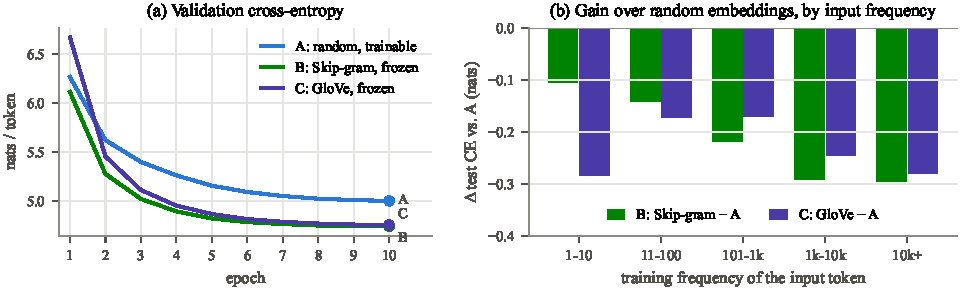
\includegraphics[width=\linewidth]{figures/fig2_part2.pdf}
\caption{Part II. (a) Validation CE per epoch. (b) Change in test CE relative to A, grouped by how often
the \emph{input} token (the one before the target) occurs in training (bucket shares of test targets:
3\%, 14\%, 24\%, 15\%, 36\%).}
\label{fig:part2}
\end{figure}

\textbf{Results} (Table~\ref{tab:part2}, Figure~\ref{fig:part2}). \obs{} Both frozen pre-trained tables beat
the jointly learned one by a wide margin ($-0.24$ / $-0.23$ nats, 20--22\% lower PPL); B and C are within
0.013 nats. \emph{Convergence}: B leads from the first epoch; C starts slowest (val PPL 790 after epoch 1)
but overtakes A during epoch 2 and approaches B every epoch. \emph{Stability}: no setting shows spikes or
non-finite gradients; maximum gradient norms are 1.8--2.2, so stability does not separate them here.
\emph{Fit}: the frozen models reach a much \emph{lower} training CE with fewer trainable parameters and also
generalise better, with a \emph{larger} train$-$val gap---freezing did not act mainly as a regulariser but
made the LM easier to optimise. \emph{Where the gain comes from} (Fig.~\ref{fig:part2}b): the frozen tables
help in every frequency band, most in absolute terms for frequent inputs ($-0.30$ nats for words seen
$>$10k times). GloVe is clearly best for the rarest inputs (words seen $\le$10 times: $-0.29$ vs $-0.10$
for Skip-gram), Skip-gram for frequent and mid-frequency ones. \emph{Representations}: A's learned table
groups closed classes well (months, numbers) but is noisy for many content words (nearest neighbours of
\emph{war}: \emph{fastra, ahk, mahdi}); Skip-gram gives corpus-specific topical neighbours (\emph{river}
$\to$ \emph{missouri, mississippi}); GloVe gives clean general semantic neighbours (\emph{war} $\to$
\emph{wars, conflict, battle}) (Appendix~\ref{app:nn}). \emph{Generation}: the frozen models stay closer to
the prompt (``scientists have found that the'' $\to$ species, kakapo, allosaurus; A drifts to a film
soundtrack); C repeats most (3.8\% repeated trigrams vs 1.3\% B, 0.4\% A).

\textbf{Interpretation: trainability vs.\ extra data.} \emph{A vs B} (same 2.08M tokens, trainable vs
pre-trained-and-frozen): under our 10-epoch budget, end-to-end trainability did not pay off; a 30-second
Skip-gram pass plus freezing was worth 0.24 nats. \hyp{} Each embedding row only receives gradient when its
word occurs, so most of the 28.9k rows get few noisy updates in 5k steps, whereas Skip-gram is built to learn
exactly these vectors from co-occurrence. \emph{B vs C} (both frozen; $\approx$2,900$\times$ more general-domain
data, but 7.5\% of test tokens without a real vector): a tie overall; the extra data helps exactly where it
should---rare words---while in-domain Skip-gram wins on frequent words. More data is not automatically better
when the small corpus \emph{is} the target domain. \emph{Not separable here}: whether the gain comes from the
pre-trained \emph{initialisation} or from \emph{freezing}; a fourth run with Skip-gram initialisation and
trainable embeddings would answer this.

\section{Part III: downstream topic classification}
\textbf{Task and protocol.} AG News \citep{zhang2015} (4 balanced news topics). From the official training
set we draw a balanced 20,000-document training set and a disjoint 5,000-document validation set (seed 42);
the official 7,600-document test set is used once. Text is preprocessed like WikiText (HTML entities removed,
lower-cased, \texttt{1 @,@ 000}, \texttt{long @-@ term}, \texttt{wasn 't}, punctuation split, \texttt{<eos>}
appended); 6.8\% of tokens fall outside the LM vocabulary and become \texttt{<unk>}; documents average 45
tokens (17 test documents exceed the 128-token context and are truncated). All five LMs stay frozen.
\textbf{Fixed-length representations}: \emph{mean} = average of the top-layer token states over the
document's real tokens (padding excluded); \emph{last} = the top-layer state at the final \texttt{<eos>},
the only position of these causal models that has read the whole document. Baselines: the average of
input-embedding rows (no context), and TF-IDF uni+bigrams over the original words (no LM, no \texttt{<unk>}).
\textbf{Classifier} (identical for all): standardised features + multinomial logistic regression
(scikit-learn \citep{pedregosa2011}), $C\in\{0.01,0.1,1,10\}$ chosen on validation accuracy; metrics: test
accuracy and macro-F1 (they agree within 0.006 because classes are balanced).

\begin{table}[!htb]
\centering\small
\caption{Part III: AG News test results with 20k training documents (chance 0.25). Validation and test
accuracy agree within 1.2 points for every row. ``Emb.\ avg'': mean of the input-embedding rows (no context).}
\label{tab:part3}
\begin{tabular}{lrcccc}
\toprule
\multirow{2}{*}{Representation} & \multirow{2}{*}{LM test PPL} & \multicolumn{2}{c}{Mean pooling} & \multicolumn{2}{c}{Last token}\\
\cmidrule(lr){3-4}\cmidrule(lr){5-6}
 & & Acc. & Macro-F1 & Acc. & Macro-F1\\
\midrule
RNN & 214.2 & 0.661 & 0.659 & 0.399 & 0.394\\
LSTM (random emb.) & 138.4 & 0.719 & 0.718 & 0.617 & 0.615\\
Transformer & 140.5 & 0.780 & 0.779 & 0.769 & 0.768\\
LSTM + Skip-gram (frozen) & 108.6 & 0.809 & 0.808 & 0.785 & 0.785\\
LSTM + GloVe (frozen) & 110.1 & \textbf{0.848} & \textbf{0.847} & \textbf{0.820} & \textbf{0.820}\\
\midrule
Emb.\ avg: LSTM's learned table / Skip-gram / GloVe & -- & \multicolumn{4}{l}{0.761 / 0.828 / 0.878 \quad (macro-F1 0.760 / 0.827 / 0.878)}\\
TF-IDF uni+bigrams (no LM) & -- & \multicolumn{4}{l}{\textbf{0.900} \quad (macro-F1 0.900)}\\
\bottomrule
\end{tabular}
\end{table}

\begin{figure}[!htb]
\centering
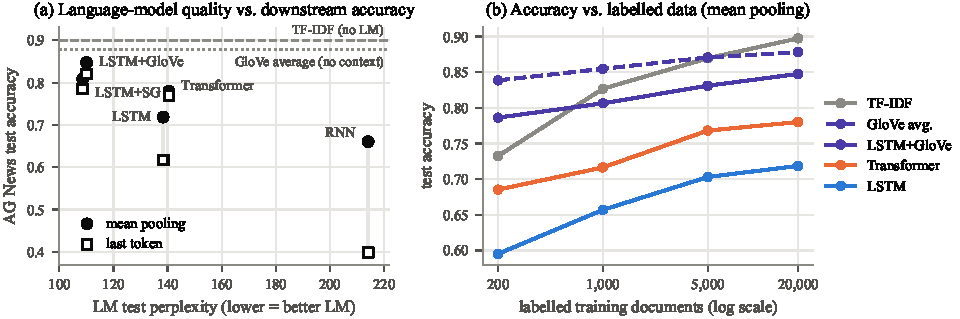
\includegraphics[width=\linewidth]{figures/fig3_part3.pdf}
\caption{Part III. (a) LM test perplexity vs.\ AG News test accuracy for both poolings (vertical segments
join the two poolings of one LM). (b) Test accuracy vs.\ number of labelled training documents (balanced
prefixes of the training set; $C$ re-selected on the same validation set).}
\label{fig:part3}
\end{figure}

\textbf{Does the LM ranking agree with the downstream ranking?} Only partly (Table~\ref{tab:part3},
Fig.~\ref{fig:part3}a). \obs{} Spearman's $\rho$ between LM test PPL and accuracy is $-0.80$ for both
poolings ($n{=}5$, $p{=}0.10$): the worst LM gives the worst features and the two frozen-embedding LSTMs the
best. But where perplexities tie, downstream accuracy does not: the Transformer beats the LSTM by 6.1 points
(mean) and 15.1 (last), and LSTM+GloVe beats LSTM+Skip-gram by 3.9 points although its PPL is slightly worse.
The downstream order follows the embedding source and the architecture more than PPL.

\textbf{Pooling and context.} \obs{} Mean pooling beats last-token pooling for every LM, by 26.2 points for
the RNN (whose final state is near chance: 39.9\%), 10.1 for the LSTM, 2.4--2.7 for the frozen-embedding LSTMs
and 1.1 for the Transformer, whose last position attends to every token directly. Strikingly, for every LSTM
the \emph{context-free} average of its own input embeddings beats its mean-pooled hidden states (GloVe 87.8 vs
84.8; Skip-gram 82.8 vs 80.9; learned 76.1 vs 71.9), although the hidden states are larger (512-d vs 300-d);
the Transformer's states (78.0) do beat the LSTM's learned-table average. \hyp{} Recurrent layers trained only
for next-word prediction re-encode their input around local, predictive information and lose some
linearly accessible topic information; the Transformer's residual stream carries each token's embedding to the
top layer and keeps more lexical identity. GloVe's advantage downstream (but not in PPL) fits its training on
general newswire-like text, whose geometry encodes topical similarity.

\textbf{Amount of labelled data} (Fig.~\ref{fig:part3}b). \obs{} With 200 labelled documents, GloVe averages
(83.8\%) and GloVe-LSTM states (78.6\%) beat TF-IDF (73.2\%) by a wide margin; TF-IDF catches up at about
5,000 documents and wins at 20,000 (89.7--90.0\%). Pre-trained dense representations matter most when labels
are scarce.

\textbf{Errors.} \obs{} Business$\leftrightarrow$Sci/Tech is the dominant confusion for every representation
(515 of the 1,159 errors of LSTM+GloVe/mean; 338 of 759 for TF-IDF), e.g.\ ``AOL to cut 700 jobs'' (Business,
predicted Sci/Tech) or ``Dell may soon unveil more consumer goods'' (Sci/Tech, predicted Business;
Table~\ref{tab:err}); some labels are debatable (a Sony/IBM chip announcement labelled Business; a cricket test match labelled World), and 224
test documents are misclassified by every LM representation. TF-IDF is right where the best LM representation
is wrong for 621 documents (221 the other way); these typically hinge on one decisive word or source tag
(\emph{ESPN}, \emph{NBA}, \emph{VoIP}, \emph{AFP}---the last is \texttt{<unk>} for the LM), which a 45-token
average dilutes. The LM representation wins on documents without a keyword but with clear topical vocabulary
(``Canada defends submarine fleet'', ``pass interference on a pivotal interception''). The share of
\texttt{<unk>} tokens barely matters (83.4--85.2\% accuracy from 0\% to $>$10\% \texttt{<unk>}).

\begin{table}[!htb]
\centering\small
\caption{Part III: representative test errors of the best LM representation (LSTM+GloVe, mean pooling)
and of TF-IDF.}
\label{tab:err}
\begin{tabular}{p{0.085\linewidth}p{0.15\linewidth}p{0.69\linewidth}}
\toprule
True & LSTM+GloVe / TF-IDF & Text (truncated)\\
\midrule
Sci/Tech & Business / \textbf{Sci/Tech} & Dell May Soon Unveil More Consumer Goods (Reuters) \ldots\ the world's largest PC maker, could announce an expanded selection of its consumer electronics line \ldots\\
Sports & Sci/Tech / \textbf{Sports} & ESPN.com news services: Six months ago, Scottie Pippen issued a ``This is probably it for me'' declaration \ldots\ in an NBA uniform.\\
World & \textbf{World} / Sports & Canada defends submarine fleet: Canada has defended its decision to buy second-hand submarines after a crewman died \ldots\\
Sports & \textbf{Sports} / World & SEC's Gaston Admits Official Missed Call (AP) \ldots\ an LSU player should have been called for pass interference on a pivotal interception \ldots\\
Business & Sci/Tech / Sci/Tech & Sony, IBM, Toshiba Give Details of `Cell' Chip (Reuters) \ldots\ (missed by every representation; debatable label)\\
World & Sports / Sports & Warne takes six but India establish handy lead (Reuters) \ldots\ (missed by every representation; debatable label)\\
\bottomrule
\end{tabular}
\end{table}

\section{Discussion, limitations and lessons}
\textbf{Across parts.} Perplexity is a good summary of next-token prediction but a coarse proxy for other
qualities: two LM pairs with tied PPL differ clearly in sample repetition (Part~I: LSTM vs Transformer) and in
downstream accuracy (Part~III: by 4--6 points). The single most effective change in this study was not the
architecture but the input embeddings: a cheap in-domain Skip-gram table, frozen, improved PPL by 22\% (Part~II),
and the representation that transferred best downstream was the one built on GloVe, whose extra data shows up
on rare words (Part~II) and on news topics (Part~III).

\textbf{Limitations.}
\begin{itemize}
\item One seed per configuration: differences below $\sim$0.02 nats or $\sim$1 accuracy point are not
  interpretable (e.g.\ LSTM vs Transformer PPL, Skip-gram vs GloVe PPL, RNN vs 4-gram).
\item Unequal tuning: two LRs for the recurrent models, one for the Transformer, and dropout 0.3 vs 0.2; hence
  ``LSTM $\approx$ Transformer'' rather than a ranking. The Part~II LR was tuned for setting A only.
\item A short 10-epoch budget favours fast-converging models; the chunked evaluation (no state across 128-token
  chunks) makes our PPLs incomparable with published WikiText-2 numbers.
\item Part~III uses frozen LMs and a linear classifier only; its 5-point correlation conflates architecture and
  embedding source; the LM vocabulary turns 6.8\% of AG News tokens into \texttt{<unk>}, which favours TF-IDF.
\item Laptop timings drift with temperature, sleep and power source.
\end{itemize}
\textbf{Lessons.}
\begin{itemize}
\item Cross-check logged metrics against an independent re-evaluation: it exposed a framework bug that had
  inverted a conclusion.
\item Report the training recipe together with the architecture: a factor-3 LR change moved the LSTM by 48 PPL.
\item For causal LMs, prefer mean pooling, and always check simple baselines: an average of good word vectors beat
  every contextual LM representation in this setting.
\end{itemize}

\small
\begin{thebibliography}{99}
\bibitem[Merity et~al.(2016)]{merity2016} S.~Merity, C.~Xiong, J.~Bradbury, R.~Socher. Pointer sentinel mixture models. \emph{arXiv:1609.07843}, 2016.
\bibitem[Kneser and Ney(1995)]{kneser1995} R.~Kneser, H.~Ney. Improved backing-off for m-gram language modeling. \emph{ICASSP}, 1995.
\bibitem[Chen and Goodman(1999)]{chen1999} S.~F.~Chen, J.~Goodman. An empirical study of smoothing techniques for language modeling. \emph{Computer Speech \& Language} 13(4), 1999.
\bibitem[Hochreiter and Schmidhuber(1997)]{hochreiter1997} S.~Hochreiter, J.~Schmidhuber. Long short-term memory. \emph{Neural Computation} 9(8), 1997.
\bibitem[Vaswani et~al.(2017)]{vaswani2017} A.~Vaswani et~al. Attention is all you need. \emph{NeurIPS}, 2017.
\bibitem[Mikolov et~al.(2013)]{mikolov2013} T.~Mikolov, I.~Sutskever, K.~Chen, G.~Corrado, J.~Dean. Distributed representations of words and phrases and their compositionality. \emph{NeurIPS}, 2013.
\bibitem[Pennington et~al.(2014)]{pennington2014} J.~Pennington, R.~Socher, C.~D.~Manning. GloVe: Global vectors for word representation. \emph{EMNLP}, 2014.
\bibitem[Zhang et~al.(2015)]{zhang2015} X.~Zhang, J.~Zhao, Y.~LeCun. Character-level convolutional networks for text classification. \emph{NeurIPS}, 2015.
\bibitem[Loshchilov and Hutter(2019)]{loshchilov2019} I.~Loshchilov, F.~Hutter. Decoupled weight decay regularization. \emph{ICLR}, 2019.
\bibitem[Paszke et~al.(2019)]{paszke2019} A.~Paszke et~al. PyTorch: An imperative style, high-performance deep learning library. \emph{NeurIPS}, 2019.
\bibitem[\v{R}eh\r{u}\v{r}ek and Sojka(2010)]{rehurek2010} R.~\v{R}eh\r{u}\v{r}ek, P.~Sojka. Software framework for topic modelling with large corpora. \emph{LREC Workshop on New Challenges for NLP Frameworks}, 2010.
\bibitem[Pedregosa et~al.(2011)]{pedregosa2011} F.~Pedregosa et~al. Scikit-learn: Machine learning in Python. \emph{JMLR} 12, 2011.
\end{thebibliography}
\normalsize

\appendix
\section{Configuration and reproducibility}\label{app:config}
\begin{table}[h]
\centering\small
\begin{tabular}{p{0.14\linewidth}p{0.40\linewidth}p{0.36\linewidth}}
\toprule
 & RNN / LSTM & Transformer\\
\midrule
Input embedding & 300-d, U($-$0.1, 0.1), trainable (Part II: frozen B/C) & same\\
Body & 2 layers, hidden 512 (LSTM: one \texttt{nn.LSTM} per layer) & 4 pre-LN blocks, 6 heads, FFN 1200, GELU, learned positions\\
Dropout & 0.3 (embedding, between layers, before softmax) & 0.2\\
Output & untied linear, 28,913 classes & untied linear\\
Peak LR & RNN 1e-3, LSTM 3e-3 (validation-selected) & 5e-4\\
\midrule
Shared & \multicolumn{2}{l}{context 128, batch 32, 10 epochs, AdamW \citep{loshchilov2019} wd 0.01, 200 warm-up steps, cosine to 10\%, clip 1.0, seed 42}\\
\bottomrule
\end{tabular}
\end{table}
Commands, configurations, random seeds and data-access instructions are in the repository's
\texttt{README.md} (PyTorch \citep{paszke2019}, gensim, scikit-learn). Each run stores \texttt{results.json}
(metrics, parameter counts, timings, hardware, generations) and \texttt{history.json} (per-epoch losses,
gradient norms); the per-part write-ups \texttt{PART1/2/3\_RESULTS.md} contain the complete tables
(e.g.\ per-class F1, learning-curve values, all generations) behind the numbers above.
\textbf{Data and tools.} WikiText-2 (CC BY-SA) and AG News (academic use) are downloaded by the scripts and
not redistributed; GloVe is downloaded through gensim-data. \textbf{Use of AI tools.} An AI coding assistant (Claude, Anthropic) was used to help write the code,
experiment scripts, figures and a first draft of this report. All experiments and results were checked and
interpreted by the author.

\section{Generated text}\label{app:gen}
\small
Prompt ``\emph{during the war , the army}'' (decoding as in Part~I; \texttt{/} = \texttt{<eos>}):\\[1pt]
\textbf{LSTM:} decided to leave the war . the german and ottoman regiment and the men had been reduced to the
french and 7th light horse brigade . the ship was held on 15 february 1903 . the 3rd infantry division was given
to a position \ldots\\
\textbf{Transformer:} corps , which he was sent to a new army troops . the battle of the 10th battalion was
appointed in mostar , but the 3rd battalion to attack the 1st infantry rifles regiments division of nevesinje
brigade \ldots\\[2pt]
Prompt ``\emph{scientists have found that the}'' (Part~II settings):\\[1pt]
\textbf{A random:} use of the `` man '' was not seen . the first of the film 's soundtrack , `` you are the
illinoise ! '' \ldots\\
\textbf{B Skip-gram:} presence of the species is not used to refer the word . / the noisy miner miner was also
described as the dubious in the american red cross \ldots\\
\textbf{C GloVe:} kakapo had `` the same time to have been the same of the more expensive '' than the same species
. / corythosaurus muscaria is a very common species of allosaurus \ldots\\[2pt]
Diversity over all 5 prompts for the Part~II settings (distinct-1 / distinct-2 / repeated-trigram rate):
A (= Part~I LSTM) 0.65 / 0.93 / 0.004; B 0.68 / 0.94 / 0.013; C 0.65 / 0.89 / 0.038.

\section{Nearest neighbours in the input-embedding tables (cosine)}\label{app:nn}
\noindent\begin{tabular}{@{}p{0.13\linewidth}p{0.26\linewidth}p{0.26\linewidth}p{0.26\linewidth}@{}}
\toprule
Word (train freq.) & A: learned with the LM & B: Skip-gram & C: GloVe\\
\midrule
war (1,370) & fastra, ahk, mahdi, bishopric & civil, outbreak, airbase, conflict & wars, conflict, battle, civil\\
guitar (400) & dj, asylums, saiban, pinyin & hero, drums, metallica, aerosmith & guitars, bass, vocals, piano\\
river (861) & fort, grape, creek, bundle & missouri, mississippi, platte, susquehanna & rivers, tributary, creek, valley\\
january (693) & november, october, february, june & november, march, february, april & february, december, october, november\\
three (1,976) & two, four, six, five & seven, eight, five, thirteen & four, five, two, six\\
scientists (57) & operatives, scholars, they, divines & exoplanets, nasa, resuscitation & researchers, experts, biologists\\
\bottomrule
\end{tabular}

\end{document}
